\documentclass[12pt,a4paper]{report}
\usepackage{amsthm,amssymb,amsmath}
\usepackage[top=50mm, bottom=50mm, left=50mm, right=50mm]{geometry}

\usepackage{graphicx}
\usepackage{subcaption}
\usepackage[pagebackref=false,colorlinks,linkcolor=blue,citecolor=magenta]{hyperref}


\usepackage{geometry}
\usepackage{datetime} 


\newcommand*{\BeginNoToc}{%
  \addtocontents{toc}{%
    \edef\protect\SavedTocDepth{\protect\the\protect\value{tocdepth}}%
  }%
  \addtocontents{toc}{%
    \protect\setcounter{tocdepth}{-10}%
  }%
}
\newcommand*{\EndNoToc}{%
  \addtocontents{toc}{%
    \protect\setcounter{tocdepth}{\protect\SavedTocDepth}%
  }%
}
\renewcommand{\bibname}{مراجع}
%\renewcommand{\refname}{مراجع}

%\usepackage[pagebackref=false]{hyperref}
\usepackage{tocbibind}
\usepackage{makeidx}
\makeindex
\usepackage{xepersian}
\settextfont[Scale=1.1]{B Nazanin}
% Latex 2020 2021 SetDigitFont error
\ExplSyntaxOn
\cs_set_eq:NN
\etex_iffontchar:D
\tex_iffontchar:D
\cs_undefine:N \c_one
\int_const:Nn \c_one { 1 }
\ExplSyntaxOff
\setdigitfont{Yas}
\defpersianfont\titr[Scale=1]{XB Titre}
\defpersianfont\nastaliq[Scale=1.5]{IranNastaliq}
\defpersianfont\traffic[Scale=1]{B Traffic}


\theoremstyle{definition}
\newtheorem{definition}{تعریف}[section]
\theoremstyle{theorem}
\newtheorem{theorem}[definition]{قضیه}
\newtheorem{lemma}[definition]{لم}
\newtheorem{proposition}[definition]{گزاره}
\newtheorem{corollary}[definition]{نتیجه}
\newtheorem{remark}[definition]{ملاحظه}
\theoremstyle{definition}
\newtheorem{example}[definition]{مثال}


\begin{document}
	\newgeometry{total={210mm,297mm}, left=40mm, right=40mm, top=20mm, bottom=20mm,}
	\pagenumbering{harfi}
	\thispagestyle{empty}
	\vspace*{25mm}
	\centerline{
\includegraphics[height=4cm]{./images/logos/iust.png}}

	\begin{center}
	\textbf{
		دانشکده مهندسی کامپیوتر
	}
	\\[1cm]
	\baselineskip=2cm
	{\titr
	\begin{Huge}
	تشخیص ناهنجاری با استفاده از شبکه‌های عمیق\\[1cm]
	\end{Huge}}
	{\Large 
		\textbf{
			گزارش سمینار کارشناسی ارشد\\
			در رشته مهندسی کامپیوتر-گرایش هوش مصنوعی و رباتیک
		} \\[1cm]
	}

	{\Large { 
	نام دانشجو:
	}
	\\
	{\Large  علی نادری پاریزی }
	\\[.5cm]
	{\Large  
		استاد راهنما:
	}
	\\
	{\Large دکتر محسن سریانی}
	\\[.6cm]
	}
	اردیبهشت ماه ۱۴۰۱
	\end{center}

	\newpage
		\begin{center}
		
\includegraphics[scale=1]{./images/god.png}
		\end{center}
	\newpage
	
	\newgeometry{total={210mm,297mm}, left=20mm, right=20mm, top=20mm, bottom=20mm,}
	
	\chapter*{چکیده}
	تشخیص ناهنجاری‌ مسئله مهمی است که در زمینه‌های تحقیقاتی گوناگون مورد مطالعه قرار می‌گیرد و کاربرد‌های بسیار زیادی دارد. یک نیاز مرسوم در حوزه تجزیه و تحلیل داده‌های دنیای واقعی، پی بردن به این است که بدانیم کدام نمونه‌ها از نقطه نظر تشابه رفتار و ظاهر با اکثریت نمونه‌های موجود بسیار متفاوت هستند. این تفاوت می‌تواند به دلیل خطای انداز‌ه‌گیری در هنگام جمع آوری داده‌ها باشد. گاهی اوقات این تفاوت می‌توانند نشان‌ دهنده وجود پدیده‌ای ناشناخته‌ باشد که در پشت‌پرده جامعه آماری مورد مطاالعه در حال رخ دادن است و ما از آن بی‌خبر هستیم. \\
در علم داده اصطلاح ناهنجاری به داده‌ای تعلق می‌گیرد از نقطه‌نظر یک معیار تشابه تعریف شده، میزان تشابه آن با سایر دادگان موجود بسیار کم باشد. برای مثال اگر عکس رادیولوژی فردی که بیماری ریوی دارد را با عکس‌های رادیولوژی گرفته شده از ریه افراد سالم مقایسه کنیم متوجه تفاوت این عکس با سایر عکس‌ها خواهیم شد. این عدم تشابه در دادگان، مشخص می‌کند  که فرد دچار بیماری ریوی است. درواقع پزشکان با مشاهده این عدم شباهت‌ها به وجود بیماری پی می‌برند. عمل مقایسه دادگان می‌تواند به وسیله کامپیوتر نیز انجام شود که موضوع این سمینار است.\\

در این سمینار تلاش شده روش‌های مبتنی بر یادگیری عمیق برای تشخیص ناهنجاری را برسی کنیم. از آنجا که کاربرد این موضوع در حوزه‌های گوناگون بسیار وسیع است و مقالات بسیار متعددی در رابطه با کاربردی‌های مختلف به چاپ رسیده، سعی کردیم حوزه سمینار را محدود کرده و ضمن معرفی انواع کاربرد‌های مسئله تشخیص ناهنجاری، به بررسی روش‌هایی بپردازیم که در رابطه با کاربرد پردازش تصویر و بینایی کامپیوتر هستند. با توجه به تعدد مقالات در سال‌های اخیر و وجود مقالات جامع در این حوزه بیشتر، مقالات جدید که در سال‌های  ۲۰۱۹ میلادی و بعد از آن منتشر شده‌اند را بررسی کنیم و برای باقی روش‌ها به ارجاع دهی به مقالات دیگر اکتفا کنیم.\\

	\textit{
واژه‌های کلیدی:
	}
	تشخیص ناهنجاری، پردازش تصویر، شبکه‌های عمیق

	\newpage
	\baselineskip=1cm
	\BeginNoToc
	\tableofcontents
	\listoffigures
	\listoftables
	\EndNoToc
	
	\newpage
	
	\baselineskip=.75cm
	\pagenumbering{arabic}
	%-------------------Chapter 1-----------------
	\chapter{مقدمه}
	تشخیص ناهنجاری‌\LTRfootnote{\lr{Anomaly detection}} مسئله مهمی است که در زمینه‌های تحقیقاتی گوناگون مورد مطالعه قرار می‌گیرد و کاربرد‌های بسیار زیادی دارد. یک نیاز مرسوم در حوزه تجزیه و تحلیل داده‌های دنیای واقعی، پی بردن این است که بدانیم کدام نمونه‌ها از نقطه نظر تشابه رفتار و ظاهر با اکثریت نمونه‌های موجود بسیار متفاوت هستند. این تفاوت می‌تواند به دلیل خطای انداز‌ه‌گیری در هنگام جمع آوری داده‌ها باشد. گاهی اوقات این تفاوت می‌توانند نشان‌ دهنده وجود پدیده‌ای ناشناخته‌ باشد که در پشت‌پرده جامعه آماری مورد مطاالعه در حال رخ دادن است و ما از آن بی‌خبر هستیم. 
	
	\begin{figure}[hp]
		  \begin{subfigure}{\linewidth}
			  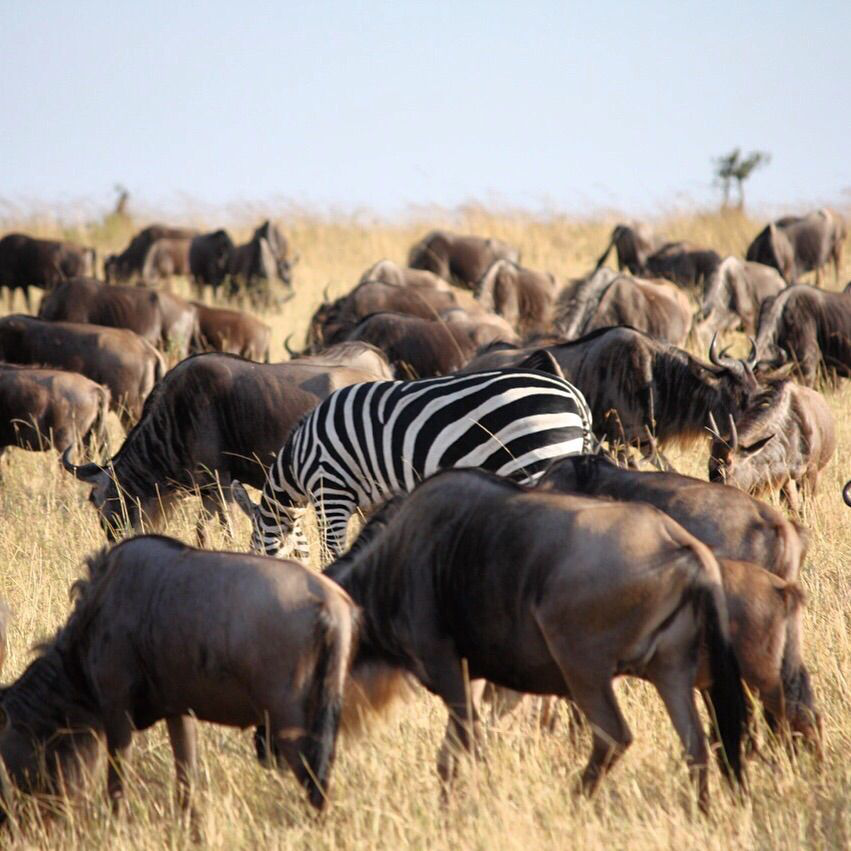
\includegraphics[width=.5\linewidth]{./images/figures/zibra-anomaly.png}\hfill
			  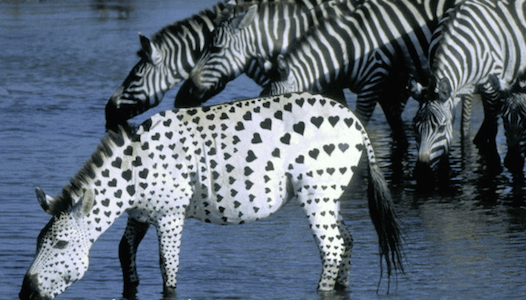
\includegraphics[width=.5\linewidth]{./images/figures/zibra-novel.png}
		  \end{subfigure}\par\medskip		  
		  \caption{مثالی از تفاوت دادگان ناهنجار و نوین}
		  \label{fig:novel-vs-anomaly}
	\end{figure}

در کنار ناهنجاری‌ها، دادگان دیگری نیز وجود دارند که با دادگان عادی متفاوت‌اند امّا این تفاوت به اندازی کافی زیاد نیست. به این دادگان اصطلاحا دادگان نوین\LTRfootnote{\lr{Novelties}} گفته می‌شود. دادگان نوین درواقع دادگانی هستند که در دسته دادگان عادی قرار می‌گیرند اما چون هنوز کشف نشده‌اند به نظر می‌رسد که با دادگان عادی تفاوت داشته باشند. برای مثال، اکثر ببر‌های دیده شده و شناخته شده به رنگ نارنجی و با خطوط راه راه سیاه هستند و دیدن بربر سفید برای ما تعجب آور خواهد بود. امّا همه به خوبی می‌دانیم که ببر سفید درواقع یک ببر است که فقط رنگ آن غیرعادی است و نباید آن را در دسته جدایی از حیوانات قرار داد.\\

در ادامه این فصل پس از تعریف ناهنجاری در دادگان، به بیان کاربرد‌های این بحث در حوزه‌های مختلف می‌پردازیم. سپس یک تعریف معیار که مرتبط با حوزه مورد نظر ما که همان پردازش تصویر است ارائه می‌دهیم. پس از تعریف حوزه مورد مطالعه و بررسی اهمیت موضوع، به توضیح ساختار کلی گزارش این سمینار خواهیم پرداخت. 
		
	\section{شرح مسئله}

   
در اکثر روش‌های ارائه شده برای تشخیص ناهنجاری اقدام به بدست آوردن یک امتیاز برای ناهنجاری\LTRfootnote{\lr{Anomaly score}} می‌کنند. این امتیاز به طریقی می‌تواند نشان‌‌دهنده احتمال تعلق این داده به دسته ناهنجاری‌ها باشد. ساده‌ترین روش برای تصمیم‌گیری در مورد یک داده قرار دادن یک مقدار آستانه برای امتیاز ناهنجاری است. اگر امتیاز داده شده به داده از مقدار آستانی بیشتر بود، داده به دسته ناهنجاری‌ها تعلق خواهد گرفت و در غیر این صورت نمی‌توان آن‌را به دسته ناهنجاری‌ها انتصاب داد.\\

اکثر روش‌های مورد استفاده برای پیدا کردن ناهنجاری‌ها در دادگان از روش‌های سنتی استفاده می‌کنند که به مراتب دارای ایراداتی هستند. با توجه به اینکه امروزه استفاده از شبکه‌های عمیق در حل مسائل رونق یافته،‌می‌توان برای حل مسئله یافتن ناهنجاری‌‌ها نیز مورد استفاده قرار گیرند. در این سمینار سعی شده روش‌های استفاده شده برای تشخیص ناهنجاری که از شبکه‌های عمیق استفاده می‌کنند را مورد بررسی قرار دهیم و ضمن معرفی انواع روش‌ها یک دسته بندی متناسب با کاربرد برای این روش‌ها نیز ارائه دهیم. با توجه به گستردگی کاربرد این حوزه، بیشتر روش‌های مورد استفاده در پردازش تصویر و بینایی کامپیوتر مورد بحث قرار خواهند گرفت.


\begin{figure}[hp]
	\begin{center}
		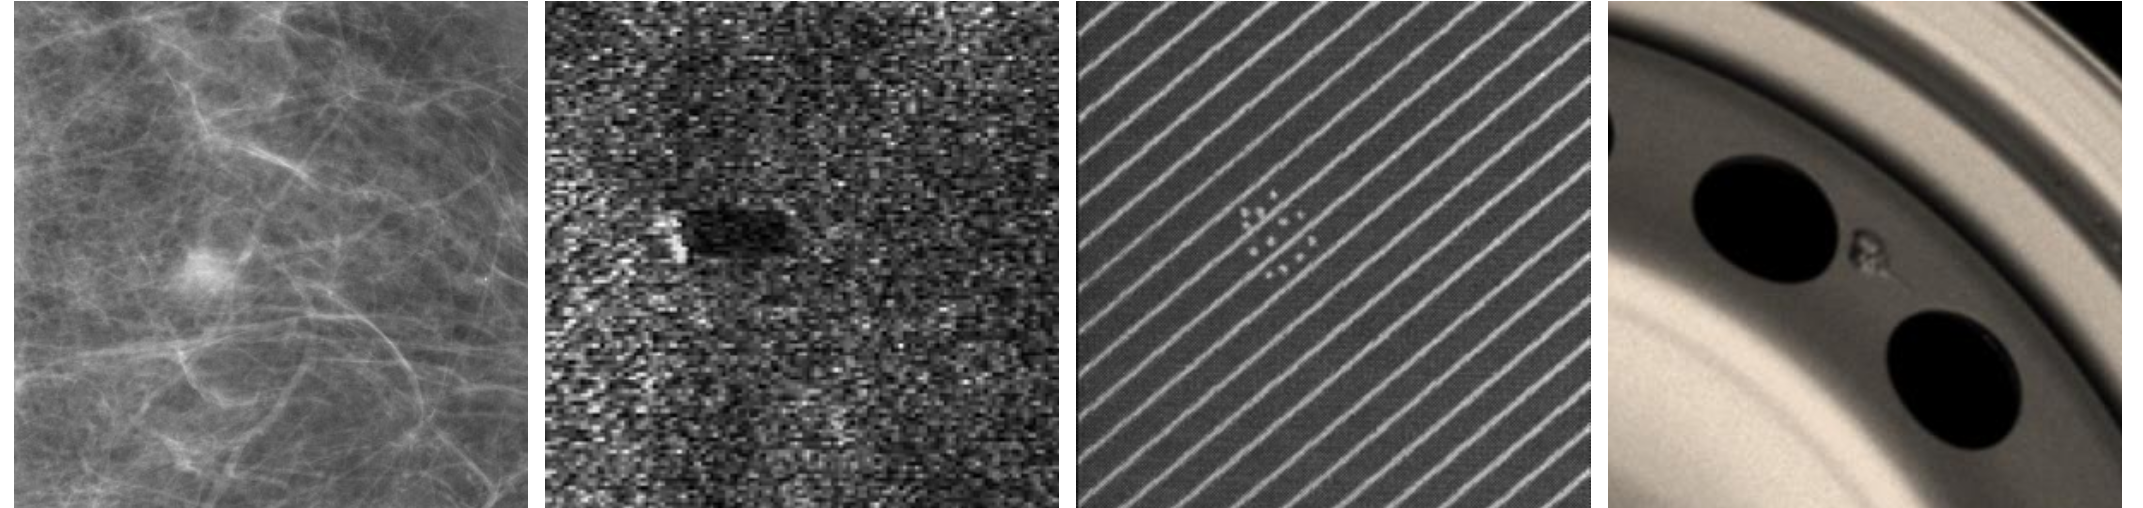
\includegraphics[width=\linewidth]{./images/figures/image-anomaly-examples-1.png}
		\caption*{به ترتیب از سمت چپ، توده سرطان سینه، مین زیر‌دریایی، نقص رنگ‌آمیزی کاشی تولید شده در کارخانه،نمونه نقص موجود در چرخ خودرو.}
		\caption{
		مثال‌هایی از ناهنجاری در تصاویر
		\cite{T.Ehret}
		}		
		\label{fig:anomaly-example-1}
		\centering
	\end{center}
\end{figure}




	\section{معرفی حوزه سمینار}


در این سمینار ابتدا یک دسته بندی کلی از روش‌های مختلف شبکه‌های عمیق ارائه کرده و سپس به بررسی روش‌های جدید که در این دسته‌بندی می‌گنجند می‌پردازیم.
در بررسی روش‌ها به کاربرد روش و مسائل قابل حل،‌پیچیدگی، قابلیت پیاده سازی صنعتی،‌نحوه آموزش و دادگان مورد نیاز خواهیم پرداخت.
	\section{اهمیت موضوع}
	
	\section{ساختار گزارش}
در فصل اوّل این سمینار به معرفی حوزه سمینار و تعریف مسئله پرداخته شد و در فصل دوّم به تعریف مفاهیم و اصطلاحات استفاده شده در این حوزه خواهیم پرداخت. فصل سوّم نیز در رابطه با بررسی کار‌های مرتبط با این سمینار و معرفی و بررسی جزئی از روش‌ها و مقالات موجود چاپ شده در سال‌های اخیر خواهد پرداخت. در ابتدای فصل سوّم پس از معرفی کار‌های مرتبط یک دسته‌بندی از روش‌های موجود ارائه می‌گردد و در ادامه، ترتیب معرفی و بررسی روش‌های موجود بر طبق این دسته‌بندی خواهد بود. در نهایت یک جمع بندی و نتیجه گیری کلی از روش‌های موجود در هر دسته انجام می‌دهیم و پیشنهاداتمان را در رابطه با استفاده از این روش‌ها بسته به کاربرد مورد نظر ارائه می‌کنیم. در فصل آخر گزارش پیشنهادات خود را درباره کار‌های آینده این حوزه ارائه کرده و در نهایت پیشنهاد انجام پروژه کارشناسی ارشد را که در راستای همین سمینار است معرفی می‌کنیم.
	%------------Chapter 2--------------
	\chapter{تعاریف و مفاهیم مبنایی}
	با توجه اهمیت یکسان بودن زبان نویسنده و خواننده برای درک مطالب پژوهش، خوب است فصلی را به بیان تعاریف و اصطلاحات رایج و پر استفاده در این سمینار اختصاص دهیم. از این رو در این بخش به معرفی و تعریف این اصطلاحات می‌پردازیم. همچنین در ادامه به معرفی و بررسی کلی الگوریتم‌های مورد استفاده در مقالات مرتبط اخیر خواهیم پرداخت تا فهم مطلب برای خوانندگان آسانتر شود. شایان ذکر است، با توجه به گستردگی مفاهیم و اصطلاحات مورد استفاده در این حوزه برای جلوگیری از زیاده‌گویی و افزایش حجم مطلب تنها اصطلاحات، تعاریف و الگوریتم‌های بسیار مرتبط در این بخش بررسی خواند شد.
	\section{اصطلاحات پرکاربرد}
		{\titr یادگیری ماشین:}\LTRfootnote{Machine learning}
		یک حوزه مطالعاتی است که در آن تمرکز بر تولید روش‌ها و الگوریتم‌هایی است که باعث شوند ماشین چیزی را یاد بگیرد.\\
		
		\noindent{\titr ناهنجاری:}\LTRfootnote{Anomaly}
در آنالیز داده،‌اصطلاح ناهنجاری به دادگانی تعلق میگیرد که با اکثریت دادگان همخوانی ندارند.\\

		\noindent{\titr یادگیری با ناظر:}\LTRfootnote{\lr{Supervised learning}}
در یادگیری ماشین هنگامی که در فرایند یادگیری دادگان برچسب خورده در اختیار داشته باشیم و یا با استفاده از یک ناظر جواب مسئله را برای هر داده بتوانیم بدست آوریم عمل یادگیری اصطلاحا یادگیری با ناظر خوانده می‌شود.
		\definition{یادگیری با نظارت ضعیف\footnote{\lr{Semi-supervised learning}}}
به عمل یادگیری گفته میشود که عمل برچسب زنی بر روی دادگان به صورت کامل انجام نگرفته است و یا بخشی از دادگان بدون برچسب صحیح در اختیار هستند.
		\definition{یادگیری بدون ناظر\footnote{\lr{Unsupervised learning}}}
نوعی از یادگیری است که در آن هیچ گونه اطلاعی از دسته بندی و یا جواب صحیح دادگان در دسترس نمی‌باشد. در این نوع از یادگیری دادگان در دسترس میتوانند به فراوانی جمع آوری شوند اما بنا به دلایلی مانند مشکل بودن فرایند برچسب زنی، برچسب دادگان در دسترس ماشین یادگیرنده قرار ندارد.
		\definition{شبکه‌های عصبی\footnote{\lr{Neural networks}}}
یک روش محاسباتی جدید است که ساختار شبکه‌ای دارد و با دریافت داده ورودی به محاسبه خروجی می‌پردازد.
		\definition{شبکه های عصبی عمیق\footnote{\lr{Deep neural networks}}}
نوعی از شبکه‌های عصبی هستند که دارای تعداد لایه‌های بیشتر از ۲ لایه هستند. این شبکه‌ها قابلیت ظرفیت یادگیری بسیار بالایی هستند و با گرفتن داده ورودی قادراند برای حل مسئله داده شده ویژگی‌های مناسب برای حل مسئله را نیز کشف کنند.
		\definition{یادگیری عمیق\footnote{\lr{Deep learning}}}
عمل یادگیری با استفاده از شبکه‌های عمیق را گویند.
		\definition{مجموعه دادگان\footnote{\lr{Dataset}}}
به مجموعه دادگان در دسترس برای انجام فرآیند یادگیری گفته میشود.
		\definition{یادگیری تقویتی\footnote{\lr{Reinforcement learning}}}
نوعی عمل یادگیری است که در آن عامل(ماشین) با محیط خود در ارتباط است و با استفاده از پاسخ‌هایی که از محیط دریافت می‌کند اقدام به یادگیری یک عمل می‌کند.
	%--------------Chapter 3--------------
	\chapter{مروری بر کار‌های مرتبط}
	\subsection{مقدمه}
	\subsection{عنوان بخش}
	\subsubsection{توضیح بخش}
	\subsection{مقایسه و نتیجه گیری}
	%-------------- Chapter 4--------------
	\chapter{نتیجه گیری و کار‌های آینده}
	\section{نتیجه گیری}
	\section{مسائل باز و کارهای قابل انجام}
	\section{موضوع پیشنهادی برای پایان نامه}
	\newpage
	
	\small
%دستوری برای ظاهر شدن کلمه«مراجع» در فهرست مطالب
\addcontentsline{toc}{section}{مراجع}
%ایجاد «مراجع»
\bibliographystyle{plain-fa}
\bibliography{bibliography.bib}


%\addcontentsline{toc}{section}{نمایه}
%دستوری برای ظاهر شدن کلمه «نمایه» در فهرست مطالب(البته در صورتی که از بسته‌ای که در ابتدا گفته شد استفاده نکرده باشید)
%ایجاد «نمایه»
\printindex
\newpage
\begin{latin}
\chapter*{Abstract}
Anomaly detection is a well studied problem in varios fileds of sciance.
% صفحه آخر ترجمه انگلیسی جلد

\newpage
\thispagestyle{empty}

	\vspace*{25mm}
	\centerline{
\includegraphics[height=4cm]{./images/logos/iust.png}}

	\begin{center}
	\textbf{
Departmant of computer engineering
	}
	\\[1cm]
	\baselineskip=2cm
	{\titr
	\begin{Huge}
	Deep learning for anomaly detection\\[1cm]
	\end{Huge}}
	{\Large 
		\textbf{
			Master seminar report \\
Computer engineering - Artificial intelligence and robotics
		} \\[1cm]
	}

	{\Large { Student name:}
	\\
	{\Large  Ali Naderi Parizi}
	\\[.5cm]
	{\Large  Professor:}
	\\
	{\Large Dr.  Mohsen Soryani}
	\\[.6cm]
	}
April 2022
	\end{center}

\end{latin}
\end{document}
